\documentclass[aspectratio=169,10pt]{beamer}
\usepackage{geometry}
\geometry{paperwidth=216mm,paperheight=121.5mm}
% Shared academic slide preamble: semantic formula colors + matching arrows.
% Copy this file with the deck. Override font directories before \input if needed.
\usepackage{fontspec,xeCJK}
\usepackage{amsmath,amssymb,booktabs,array,tabularx,tikz}
\usepackage[math-style=TeX,mathrm=sym]{unicode-math}
\providecommand{\AcademicLatinFontPath}{/home/zhuhourui/.local/share/fonts/microsoft-academic/}
\providecommand{\AcademicCJKFontPath}{/home/zhuhourui/.local/share/fonts/microsoft-academic/}
\setmainfont{Arial.TTF}[Path=\AcademicLatinFontPath,BoldFont=Arialbd.TTF,ItalicFont=Ariali.TTF]
\setsansfont{Arial.TTF}[Path=\AcademicLatinFontPath,BoldFont=Arialbd.TTF,ItalicFont=Ariali.TTF]
\setCJKmainfont{msyh.ttf}[Path=\AcademicCJKFontPath,BoldFont=msyhbd.ttf]
\setCJKsansfont{msyh.ttf}[Path=\AcademicCJKFontPath,BoldFont=msyhbd.ttf]
\setmathfont{Latin Modern Math}
\usefonttheme{professionalfonts}
\usetheme{default}
\usetikzlibrary{arrows.meta,positioning,calc}
\definecolor{MainBlue}{HTML}{1F3A5F}
\definecolor{AccentOrange}{HTML}{C97A06}
\definecolor{AccentGreen}{HTML}{008060}
\definecolor{AccentRed}{HTML}{C44E52}
\definecolor{AccentPurple}{HTML}{7A5195}
\definecolor{Ink}{HTML}{202630}
\definecolor{Muted}{HTML}{626B76}
\definecolor{SoftBlue}{HTML}{EAF2FB}
\setbeamercolor{normal text}{fg=Ink,bg=white}
\setbeamercolor{structure}{fg=MainBlue}
\setbeamercolor{frametitle}{fg=MainBlue,bg=white}
\setbeamercolor{evidence}{fg=Ink,bg=SoftBlue}
\setbeamerfont{frametitle}{size=\fontsize{17}{21}\selectfont,series=\bfseries}
\setbeamersize{text margin left=11mm,text margin right=11mm}
\setbeamertemplate{navigation symbols}{}
\setbeamertemplate{frametitle}{%
  \vspace{3mm}\begin{beamercolorbox}[wd=\textwidth,sep=0pt]{frametitle}%
  \usebeamerfont{frametitle}\insertframenumber\quad\insertframetitle\strut\par
  \end{beamercolorbox}\vspace{3mm}}
\providecommand{\AcademicFooter}{学术汇报}
\setbeamertemplate{footline}{%
  \hspace{11mm}{\color{Muted}\fontsize{8}{10}\selectfont\AcademicFooter\hfill
  \insertframenumber\,/\,\inserttotalframenumber}\hspace{11mm}\vspace{3mm}}
\renewcommand{\normalsize}{\fontsize{11}{15}\selectfont}
\AtBeginDocument{\normalsize}
\setlength{\parindent}{0pt}
\setlength{\parskip}{2mm}
\pdfstringdefDisableCommands{\def\translate#1{#1}}
\tikzset{
  term/.style={font=\fontsize{16}{20}\selectfont,inner sep=1pt},
  compact term/.style={term,font=\fontsize{13}{17}\selectfont},
  explain/.style={align=center,anchor=north,font=\fontsize{10.5}{14}\selectfont,inner sep=1pt},
  compact explain/.style={explain,font=\fontsize{9.5}{12}\selectfont},
  link/.style={-{Stealth[length=2.1mm]},thick}
}
% #1 formula node, #2 semantic color, #3 label coordinate, #4 width,
% #5 physical role, #6 short explanatory sentence. Endpoints use node anchors.
\newcommand{\termnote}[6]{%
  \node[explain,text width=#4] (#1-note) at #3
  {\textcolor{#2}{\bfseries #5}\\#6};
  \draw[link,#2] (#1.south) -- (#1-note.north);}
\newcommand{\takeaway}[1]{\par\vspace{1mm}%
  \begin{beamercolorbox}[wd=\textwidth,sep=1.4mm]{evidence}%
  \centering\fontsize{10.5}{14}\selectfont #1\end{beamercolorbox}}
\newcommand{\src}[1]{\par\vfill{\color{Muted}\fontsize{8.5}{11}\selectfont #1\par}}

\renewcommand{\AcademicFooter}{Mini-quenching 复现审计 | arXiv:2609.19265v1 | 2026-09-20}
\begin{document}
\begin{frame}[t]{本轮完成了运行与审计，完整模型尚未通过验收}
\par
\begin{tabular}{lll}
\toprule 目标 & 状态 & 实际证据\\\midrule
图 1 参数化 IMF & reproduced & 六条曲线最大相对差异 $8.55\times10^{-6}$\\
图 4 简化质量上限 & approximate & 两种原文可支持的约定仍有差异\\
图 2、5、8 全反馈 & blocked & 热学闭合缺项，部分启动无法解析\\
图 2、5、8 SN-only & approximate & 已运行；不能替代完整反馈\\
其余图 & not\_run & 按核心优先顺序，尚未进入\\\bottomrule
\end{tabular}

24 项测试通过。全反馈扫描 467 条，SN-only 扫描 499 条。

数值收敛和论文符合性分别验收；没有调整参数追逐参考曲线。
\src{原文、源码、独立矢量参考曲线与 SHA256 已保存；完整说明见 reproduction\_report.md。}
\end{frame}
\begin{frame}[t]{两处物理约定决定了如何解释主图}
\par
\[ M_{\rm enc}(r)=\frac{2\sigma^2r}{G},\qquad \sigma^2=\frac{GM_h}{r_{\rm vir}}
\quad\Rightarrow\quad g(r)=\frac{2GM_h}{r_{\rm vir}r}.\]
总质量尺度 $M_h$ 与包围质量不同；在 $r_{\rm vir}$ 得 $M_{\rm enc}=2M_h$。
基线保留式 (1)、(2)、(22) 的因子 2，并测试因子 1 的独立分支。

\[ \Phi(m)=\frac{dN}{dm}\propto m^{-\alpha}e^{-(m_{\rm char}/m)^{1.6}},
\qquad\int_{0.08}^{100}m\Phi(m)\,dm=1.\]
正文 Chabrier-like：$\alpha=2.35,\ m_{\rm char}=0.2M_\odot$。
图 1 图注的 1.35、图 5 图注的 $-2.35$ 与正文冲突；原图曲线支持正文。
\src{Luberto \& Furlanetto v1，§2.1、§2.4、§3.1；HTML 编号与 PDF 节内编号不同。}
\end{frame}
\begin{frame}[t]{图 1：单位形成质量的 IMF 校验}
\par
\begin{columns}[T,onlytextwidth]
\begin{column}{.485\textwidth}
\centering\textbf{论文原图}\\[1mm]
\begin{minipage}[c][6.65cm][c]{\linewidth}\centering
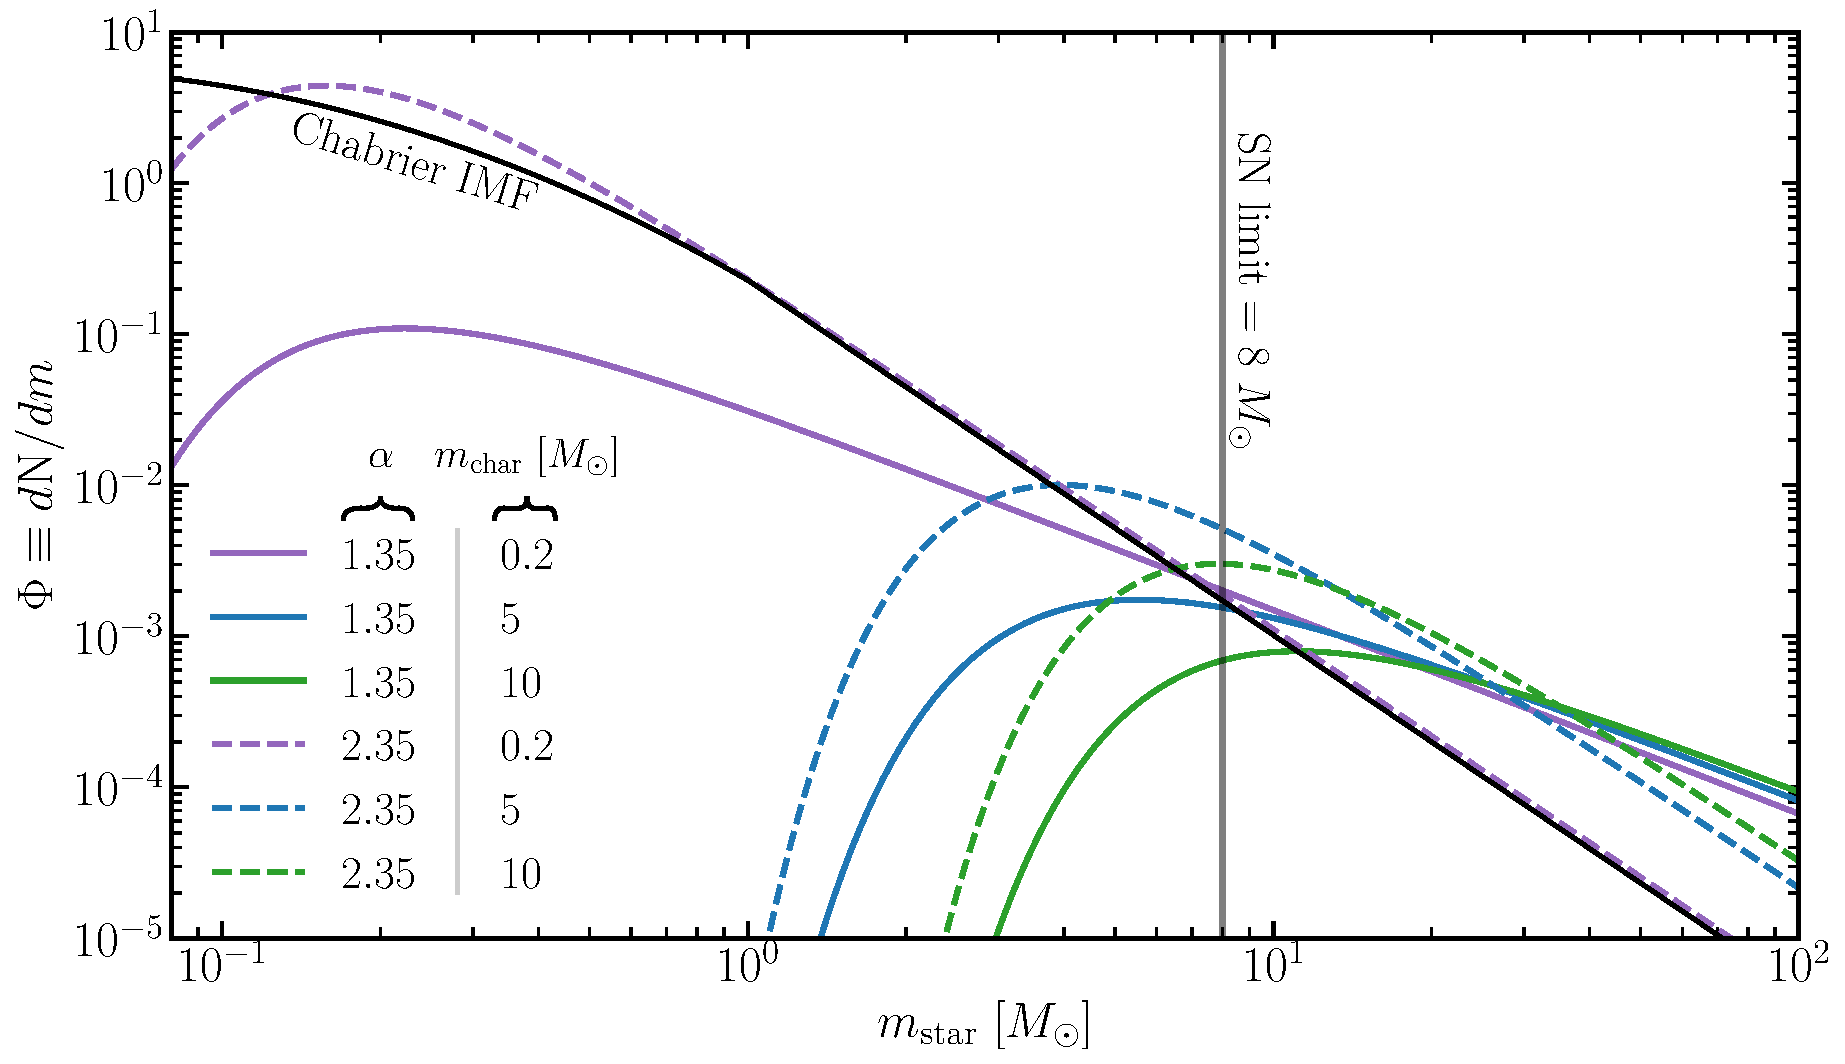
\includegraphics[width=\linewidth,height=6.6cm,keepaspectratio]{assets/comparison/fig1_original.pdf}
\end{minipage}
\end{column}
\begin{column}{.485\textwidth}
\centering\textbf{复现结果}\\[1mm]
\begin{minipage}[c][6.65cm][c]{\linewidth}\centering
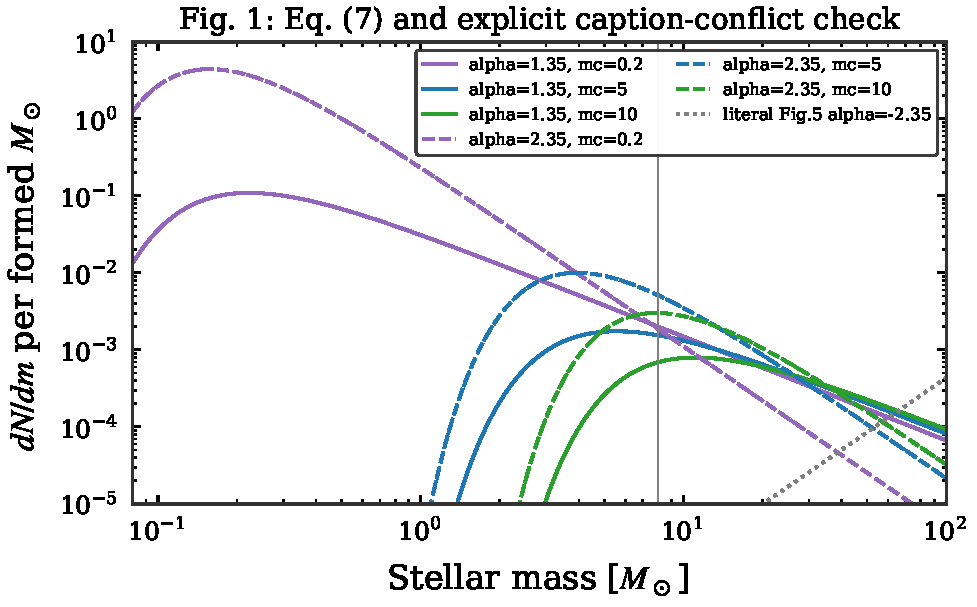
\includegraphics[width=\linewidth,height=6.6cm,keepaspectratio]{assets/figure1_imf.pdf}
\end{minipage}
\end{column}
\end{columns}
\vspace{1mm}
{\fontsize{10}{13}\selectfont 六条参数曲线最大相对差异 $8.55\times10^{-6}$；黑色经验 Chabrier 比较线未重拟合。\par}
\src{原图：Luberto \& Furlanetto v1，TeX 源包；右图来自已保存的实际计算。}
\end{frame}
\begin{frame}[t]{图 2：SN-only 诊断分支，尚未复现原图}
\par
\begin{columns}[T,onlytextwidth]
\begin{column}{.485\textwidth}
\centering\textbf{论文原图}\\[1mm]
\begin{minipage}[c][6.65cm][c]{\linewidth}\centering
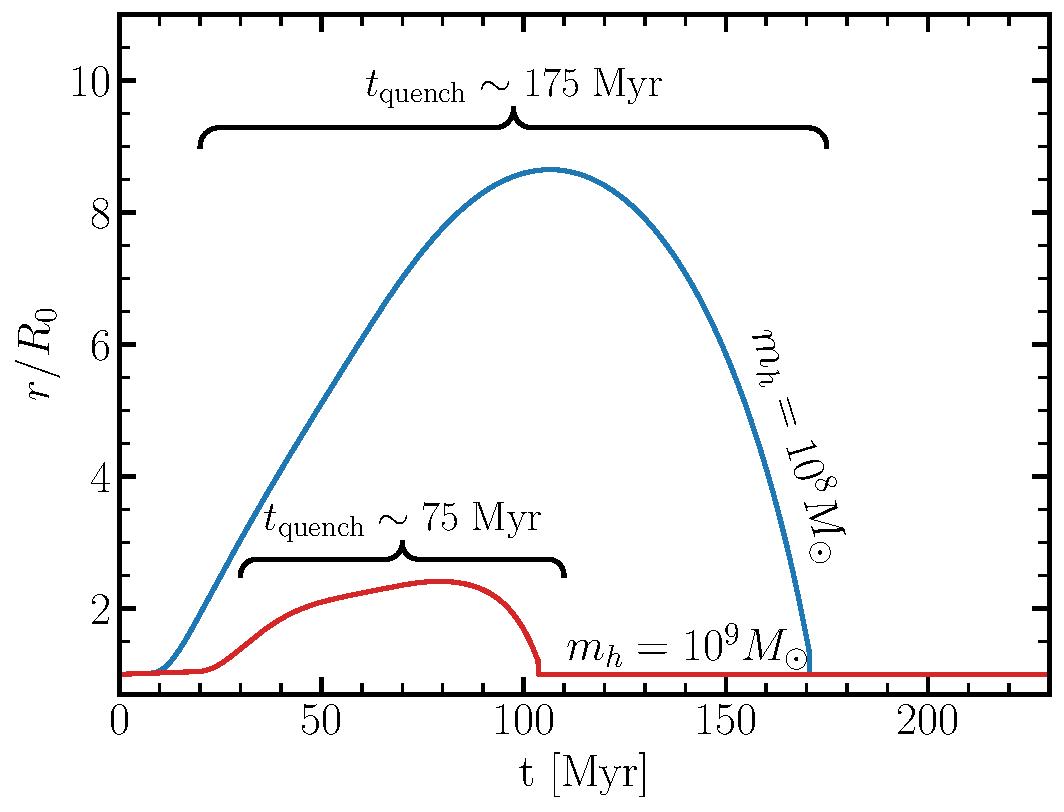
\includegraphics[width=\linewidth,height=6.6cm,keepaspectratio]{assets/comparison/fig2_original.pdf}
\end{minipage}
\end{column}
\begin{column}{.485\textwidth}
\centering\textbf{复现结果}\\[1mm]
\begin{minipage}[c][6.65cm][c]{\linewidth}\centering
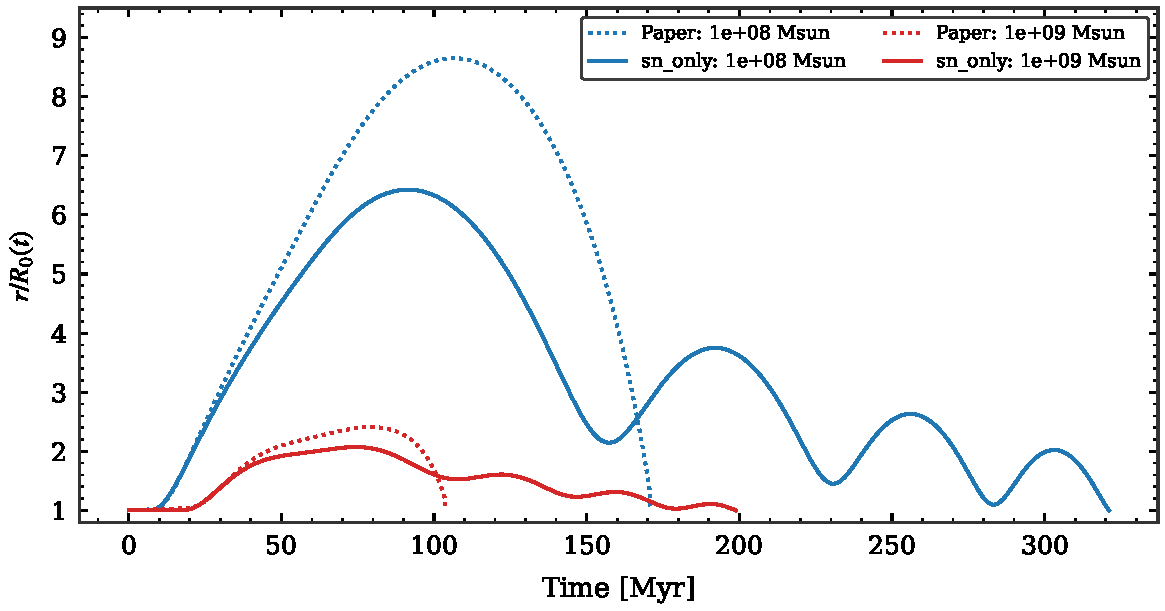
\includegraphics[width=\linewidth,height=6.6cm,keepaspectratio]{assets/review_fig2_sn_only.pdf}
\end{minipage}
\end{column}
\end{columns}
\vspace{1mm}
{\fontsize{10}{13}\selectfont $f_\star=0.001$、$f_{\rm cover}=1$；返回 $R_0(t)$ 才结束淬火。计算为 315.1/182.9 Myr，原图约 175/75 Myr。\par}
\src{原图 Fig. 2；右图 until\_return 分支，实线为计算、点线为原图取样。两侧时间范围不同。}
\end{frame}
\begin{frame}[t]{图 2 偏差诊断：回落压缩触发反弹，作者实现仍未恢复}
\par
\[ \dot P=\frac{L_{\rm SN}}{2\pi r^3}-5P\frac{v}{r}-\frac{P}{t_{\rm comp}},
\qquad v<0\ \Rightarrow\ -5Pv/r>0. \]
蓝线首次反弹约在 157.5 Myr：SFR 与 SN 率均为零，压力力约为内向合力的 1.98 倍。
已有热泡受压后再次推动壳层，延长了返回时间；这不是新一轮恒星形成。

\begin{tabular}{lll}
\toprule 检查 & 本次实测 & 能说明什么\\\midrule
蓝线加密积分 & 315.067 $\to$ 315.063 Myr & 反弹并非粗步长造成\\
仅外流加载，$10^8M_\odot$ & 390.5 Myr，5 次反弹 & 换加载分支仍未吻合\\
仅外流加载，$10^9M_\odot$ & 速度切换积分失败 & 数值处理仍有缺口\\\bottomrule
\end{tabular}

右图同时省略 UV/Ly$\alpha$，且使用回落仍加载的 until\_return 分支。
第 2.9 节的字面规则是仅外流时加载；该替代分支不能作为论文基线。
\src{压力方程：原文式 (2.16)、(2.17)。反弹机制已查明；原图不反弹的原因仍未确定，不能任意删除压缩项。}
\end{frame}
\begin{frame}[t]{图 2：全反馈近似仍受启动闭合限制}
\par
\begin{columns}[T,onlytextwidth]
\begin{column}{.485\textwidth}
\centering\textbf{论文原图}\\[1mm]
\begin{minipage}[c][6.65cm][c]{\linewidth}\centering
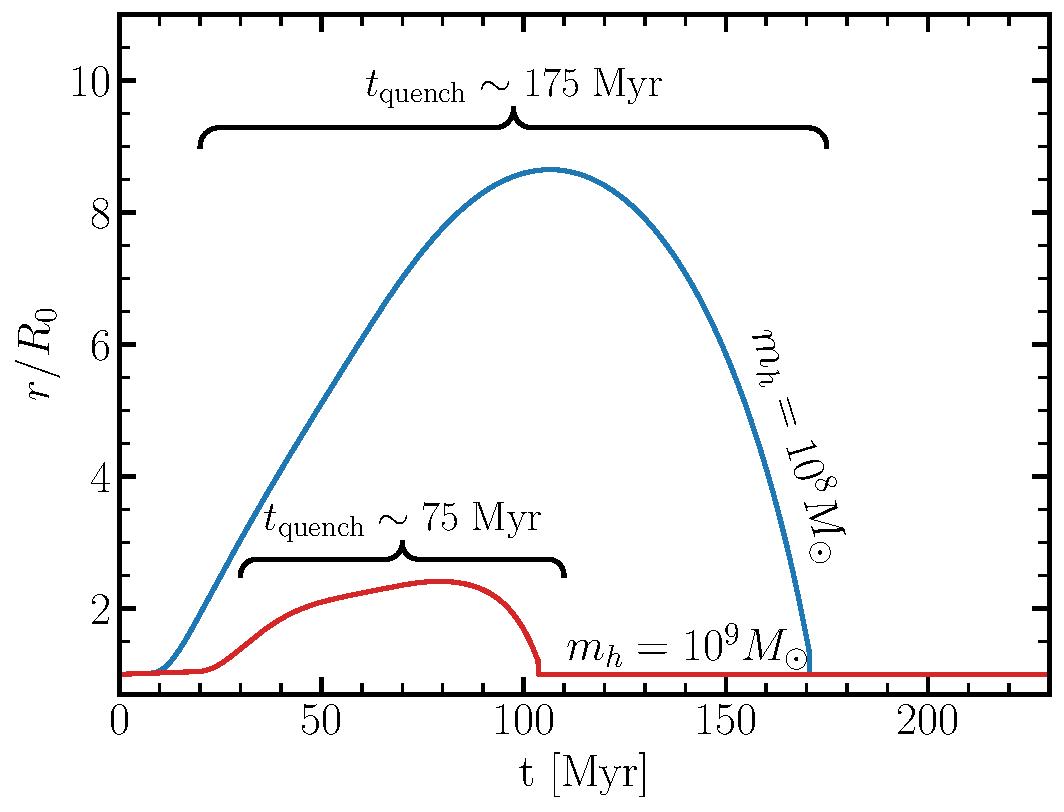
\includegraphics[width=\linewidth,height=6.6cm,keepaspectratio]{assets/comparison/fig2_original.pdf}
\end{minipage}
\end{column}
\begin{column}{.485\textwidth}
\centering\textbf{复现结果}\\[1mm]
\begin{minipage}[c][6.65cm][c]{\linewidth}\centering
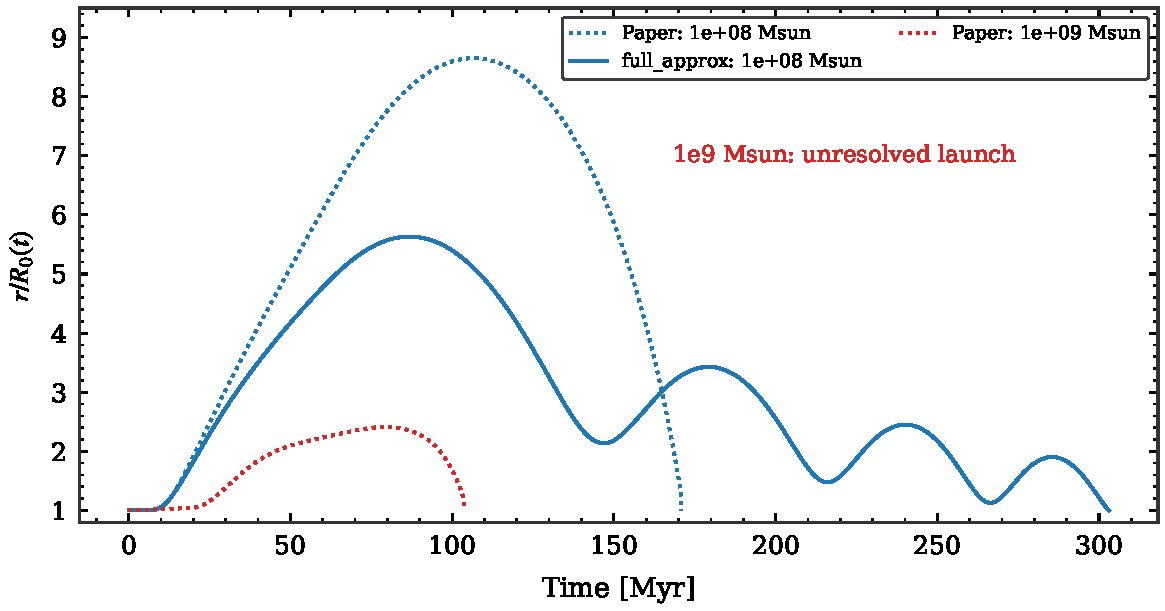
\includegraphics[width=\linewidth,height=6.6cm,keepaspectratio]{assets/review_fig2_full_approx.pdf}
\end{minipage}
\end{column}
\end{columns}
\vspace{1mm}
{\fontsize{10}{13}\selectfont full\_approx：$10^8M_\odot$ 淬火约 297.5 Myr；$10^9M_\odot$ 未得到可解析启动，保留为失败。\par}
\src{原图 Fig. 2；右图含真实 MF 拟合与冷却表，壳层密度/厚度仍为推断。点线为原图取样；时间范围不同。}
\end{frame}
\begin{frame}[t]{图 4：简化最大可淬火质量，$z=3$}
\par
\begin{columns}[T,onlytextwidth]
\begin{column}{.485\textwidth}
\centering\textbf{论文原图}\\[1mm]
\begin{minipage}[c][6.65cm][c]{\linewidth}\centering
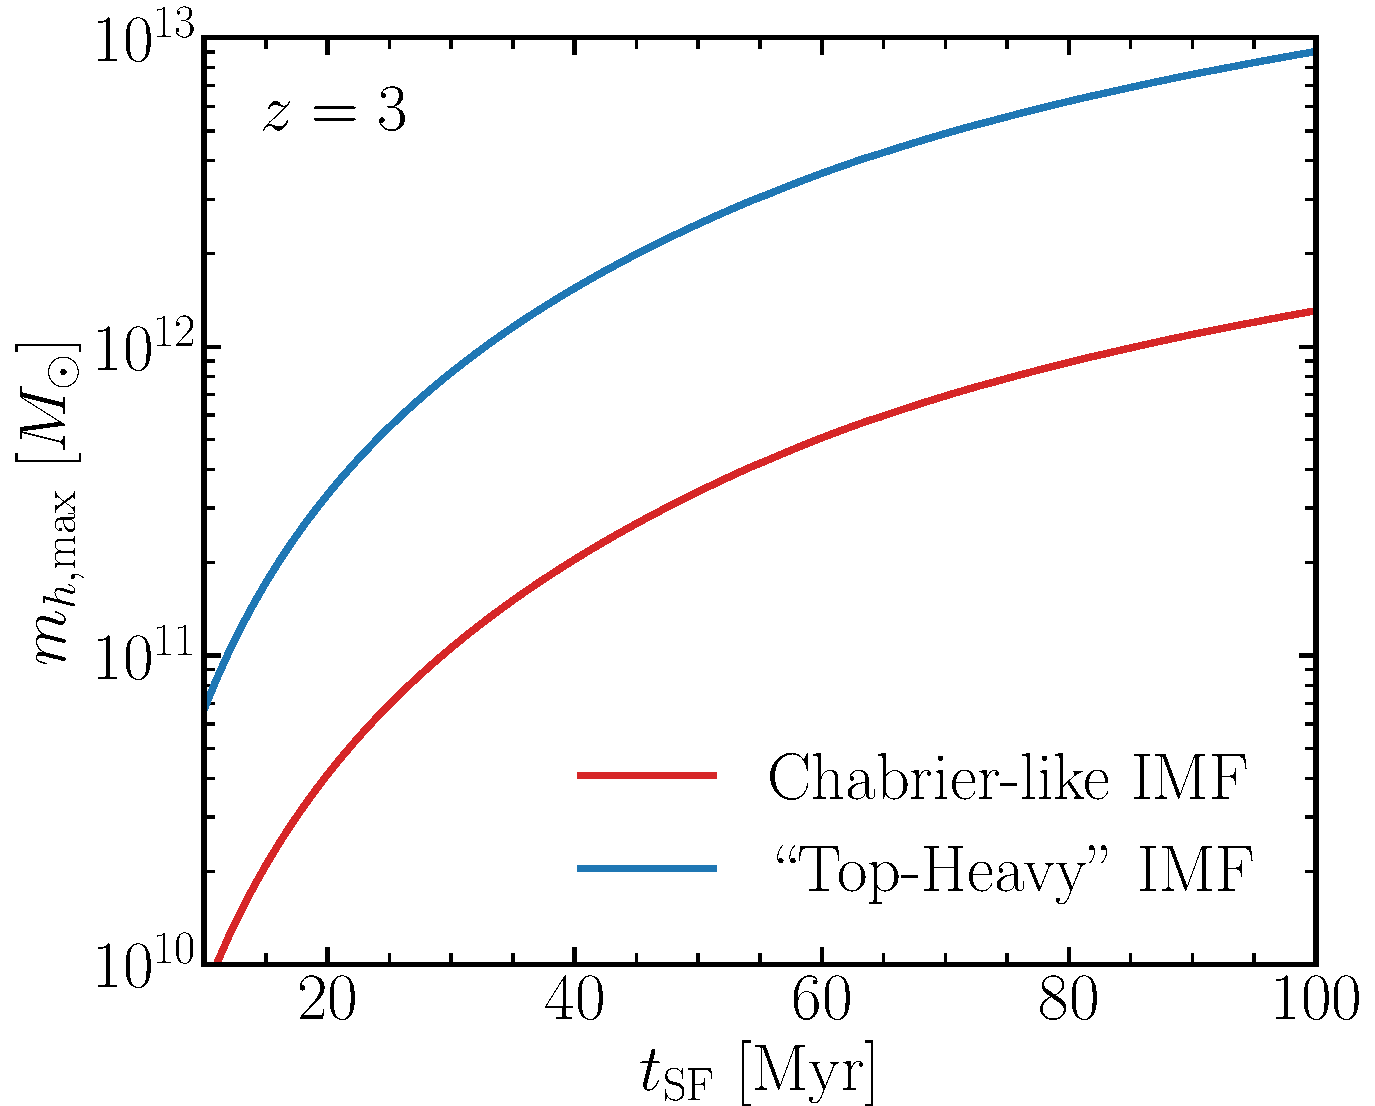
\includegraphics[width=\linewidth,height=6.6cm,keepaspectratio]{assets/comparison/fig4_z3_original.pdf}
\end{minipage}
\end{column}
\begin{column}{.485\textwidth}
\centering\textbf{复现结果}\\[1mm]
\begin{minipage}[c][6.65cm][c]{\linewidth}\centering
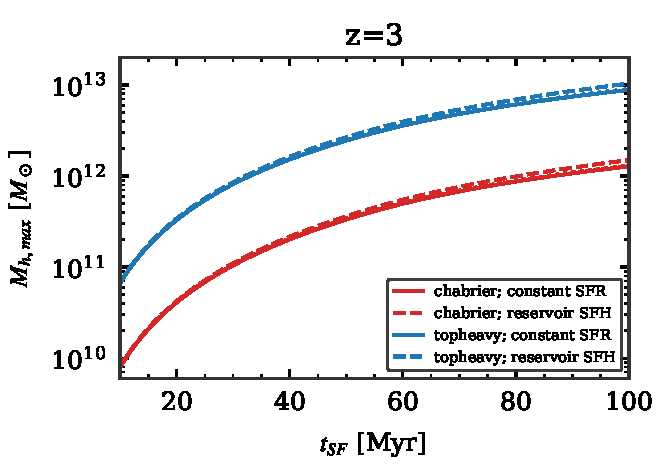
\includegraphics[width=\linewidth,height=6.6cm,keepaspectratio]{assets/comparison/fig4_z3_computed.pdf}
\end{minipage}
\end{column}
\end{columns}
\vspace{1mm}
{\fontsize{10}{13}\selectfont 红：Chabrier-like；蓝：top-heavy。右图实线为固定初始 SFR，虚线为储库 SFH，点线为原图。\par}
\src{原图 Fig. 4 对应面板裁切；黑线为式 (33)。固定 SFR 分支跨面板最大差异约 2--23\%；纵轴为 $M_{h,\max}/M_\odot$。}
\end{frame}
\begin{frame}[t]{图 4：简化最大可淬火质量，$z=6$}
\par
\begin{columns}[T,onlytextwidth]
\begin{column}{.485\textwidth}
\centering\textbf{论文原图}\\[1mm]
\begin{minipage}[c][6.65cm][c]{\linewidth}\centering
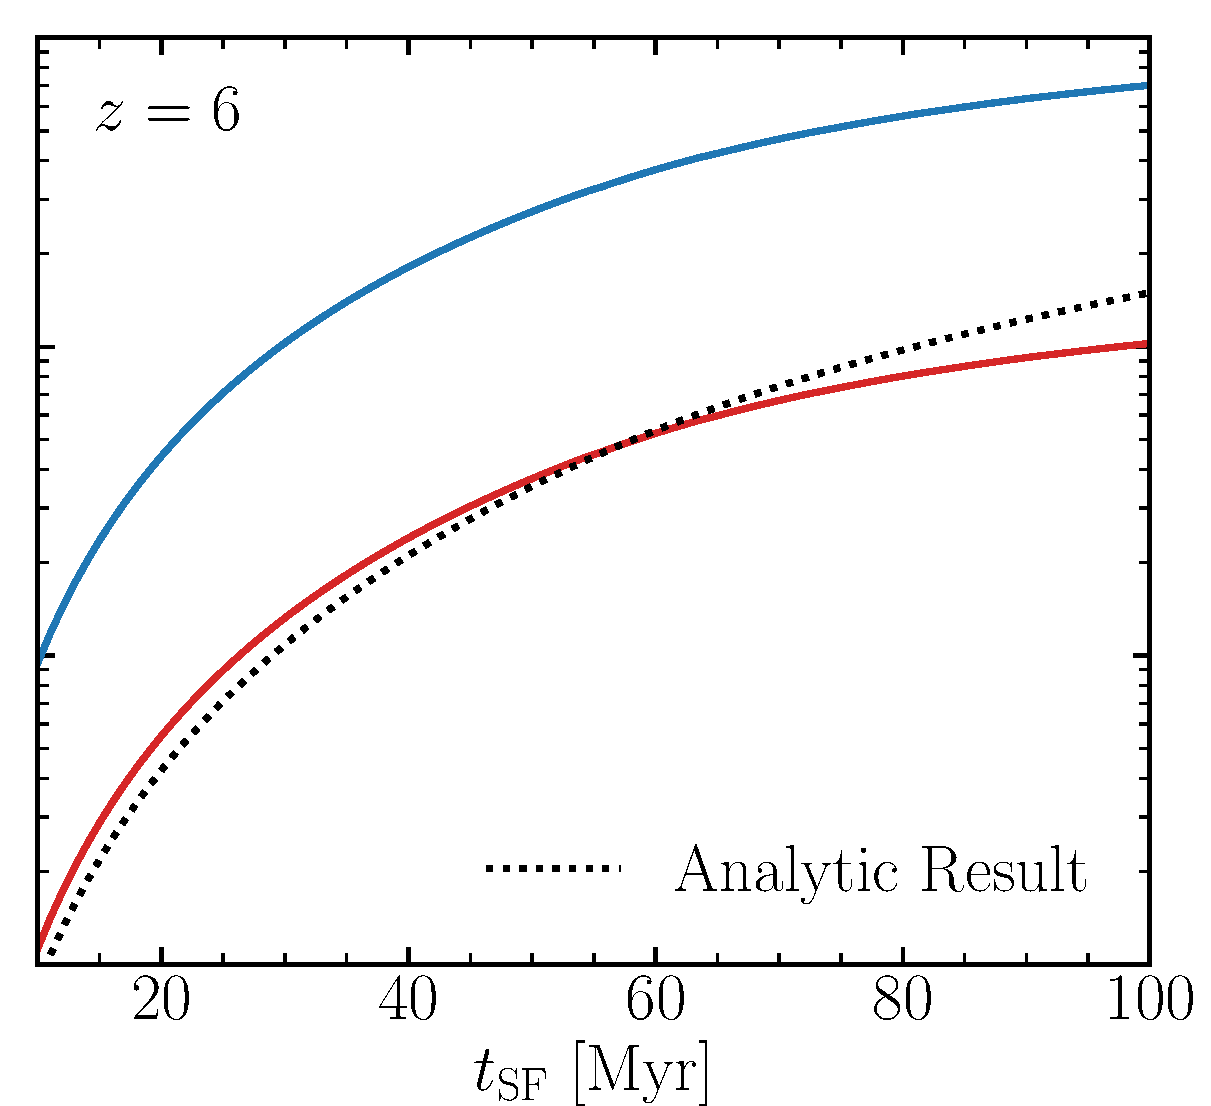
\includegraphics[width=\linewidth,height=6.6cm,keepaspectratio]{assets/comparison/fig4_z6_original.pdf}
\end{minipage}
\end{column}
\begin{column}{.485\textwidth}
\centering\textbf{复现结果}\\[1mm]
\begin{minipage}[c][6.65cm][c]{\linewidth}\centering
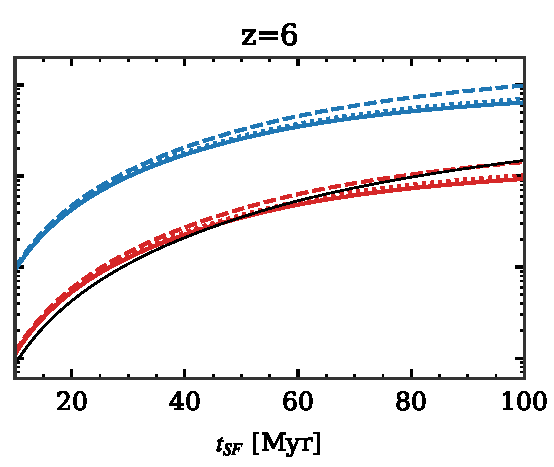
\includegraphics[width=\linewidth,height=6.6cm,keepaspectratio]{assets/comparison/fig4_z6_computed.pdf}
\end{minipage}
\end{column}
\end{columns}
\vspace{1mm}
{\fontsize{10}{13}\selectfont 红：Chabrier-like；蓝：top-heavy。右图实线为固定初始 SFR，虚线为储库 SFH，点线为原图。\par}
\src{原图 Fig. 4 对应面板裁切；黑线为式 (33)。固定 SFR 分支跨面板最大差异约 2--23\%；纵轴为 $M_{h,\max}/M_\odot$。}
\end{frame}
\begin{frame}[t]{图 4：简化最大可淬火质量，$z=9$}
\par
\begin{columns}[T,onlytextwidth]
\begin{column}{.485\textwidth}
\centering\textbf{论文原图}\\[1mm]
\begin{minipage}[c][6.65cm][c]{\linewidth}\centering
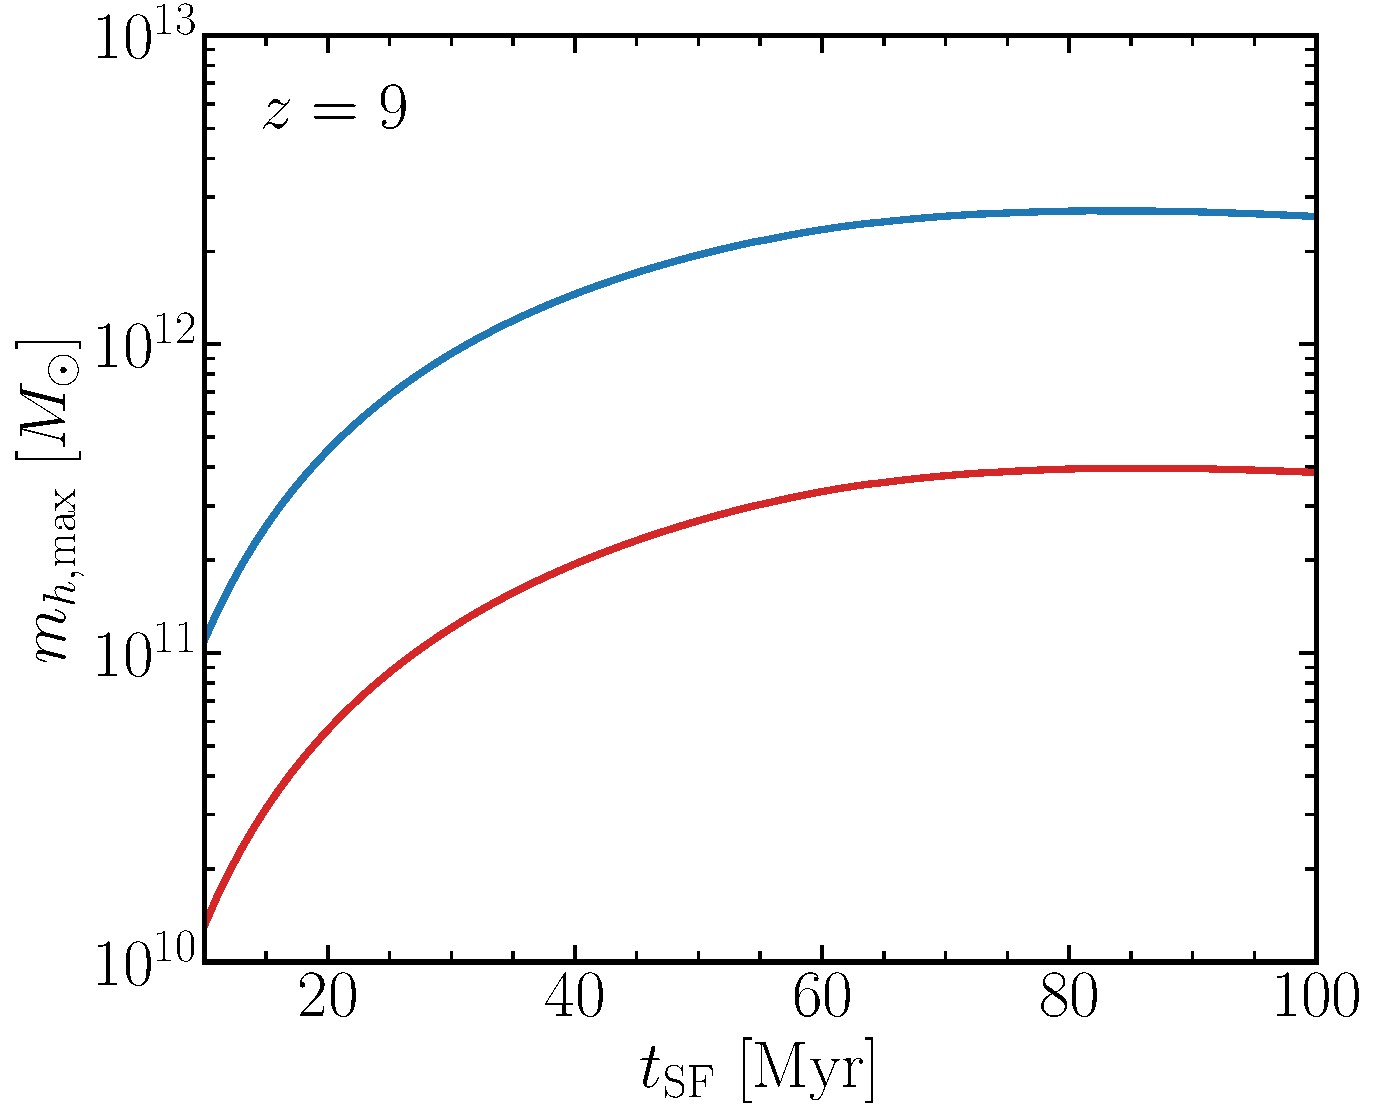
\includegraphics[width=\linewidth,height=6.6cm,keepaspectratio]{assets/comparison/fig4_z9_original.pdf}
\end{minipage}
\end{column}
\begin{column}{.485\textwidth}
\centering\textbf{复现结果}\\[1mm]
\begin{minipage}[c][6.65cm][c]{\linewidth}\centering
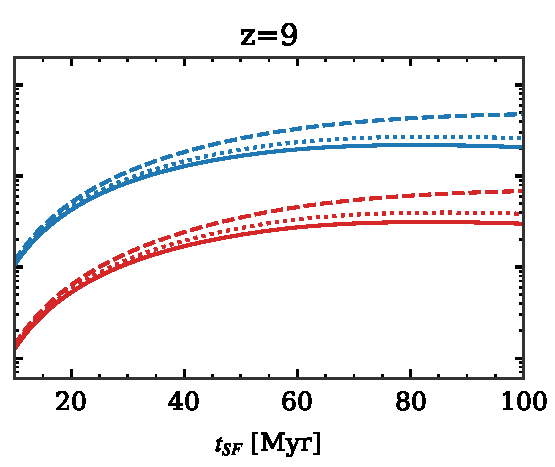
\includegraphics[width=\linewidth,height=6.6cm,keepaspectratio]{assets/comparison/fig4_z9_computed.pdf}
\end{minipage}
\end{column}
\end{columns}
\vspace{1mm}
{\fontsize{10}{13}\selectfont 红：Chabrier-like；蓝：top-heavy。右图实线为固定初始 SFR，虚线为储库 SFH，点线为原图。\par}
\src{原图 Fig. 4 对应面板裁切；黑线为式 (33)。固定 SFR 分支跨面板最大差异约 2--23\%；纵轴为 $M_{h,\max}/M_\odot$。}
\end{frame}
\begin{frame}[t]{图 5：形成效率与暗晕质量}
\par
\begin{columns}[T,onlytextwidth]
\begin{column}{.485\textwidth}
\centering\textbf{论文原图}\\[1mm]
\begin{minipage}[c][6.65cm][c]{\linewidth}\centering
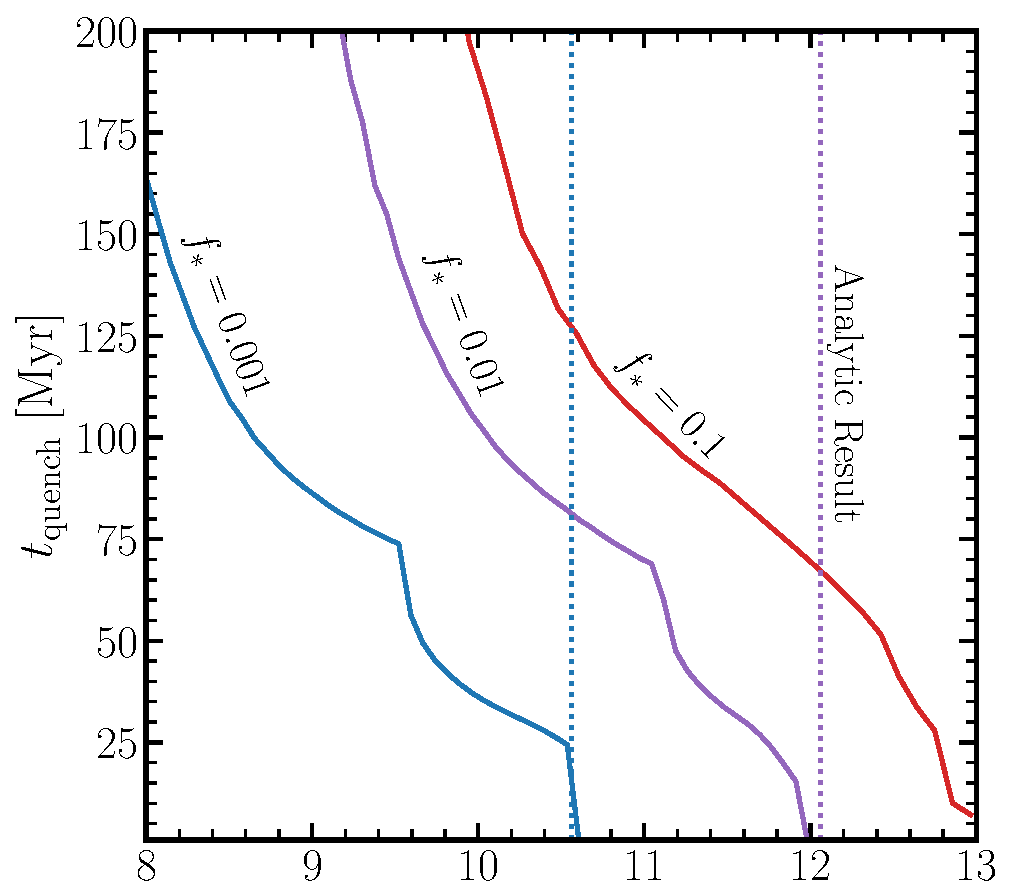
\includegraphics[width=\linewidth,height=6.6cm,keepaspectratio]{assets/comparison/fig5_eff_halo_original.pdf}
\end{minipage}
\end{column}
\begin{column}{.485\textwidth}
\centering\textbf{复现结果}\\[1mm]
\begin{minipage}[c][6.65cm][c]{\linewidth}\centering
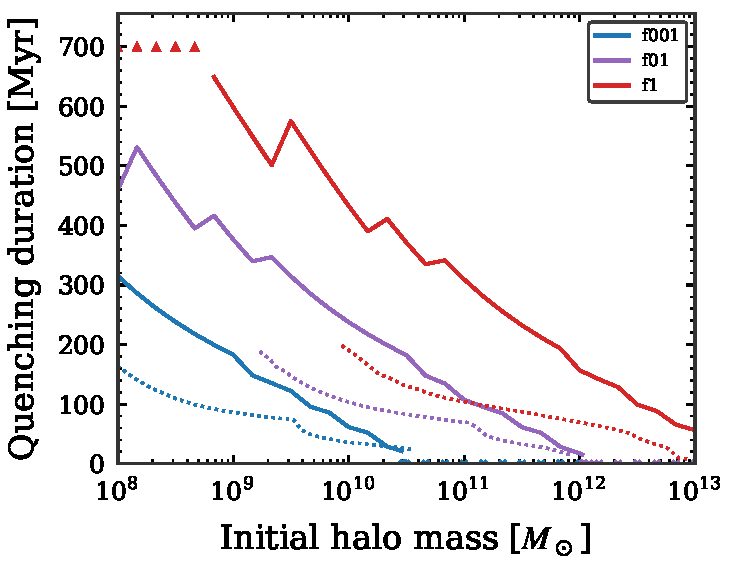
\includegraphics[width=\linewidth,height=6.6cm,keepaspectratio]{assets/comparison/fig5_eff_halo_computed.pdf}
\end{minipage}
\end{column}
\end{columns}
\vspace{1mm}
{\fontsize{10}{13}\selectfont 右图为 SN-only：f001/f01/f1 分别指 $f_\star=0.001/0.01/0.1$。点线为原图取样。\par}
\src{原图 Fig. 5 对应面板裁切；左右纵轴范围不同。右侧叉号为未启动、红短线为失败、三角为未返回下限。}
\end{frame}
\begin{frame}[t]{图 5：形成效率与观测恒星质量映射}
\par
\begin{columns}[T,onlytextwidth]
\begin{column}{.485\textwidth}
\centering\textbf{论文原图}\\[1mm]
\begin{minipage}[c][6.65cm][c]{\linewidth}\centering
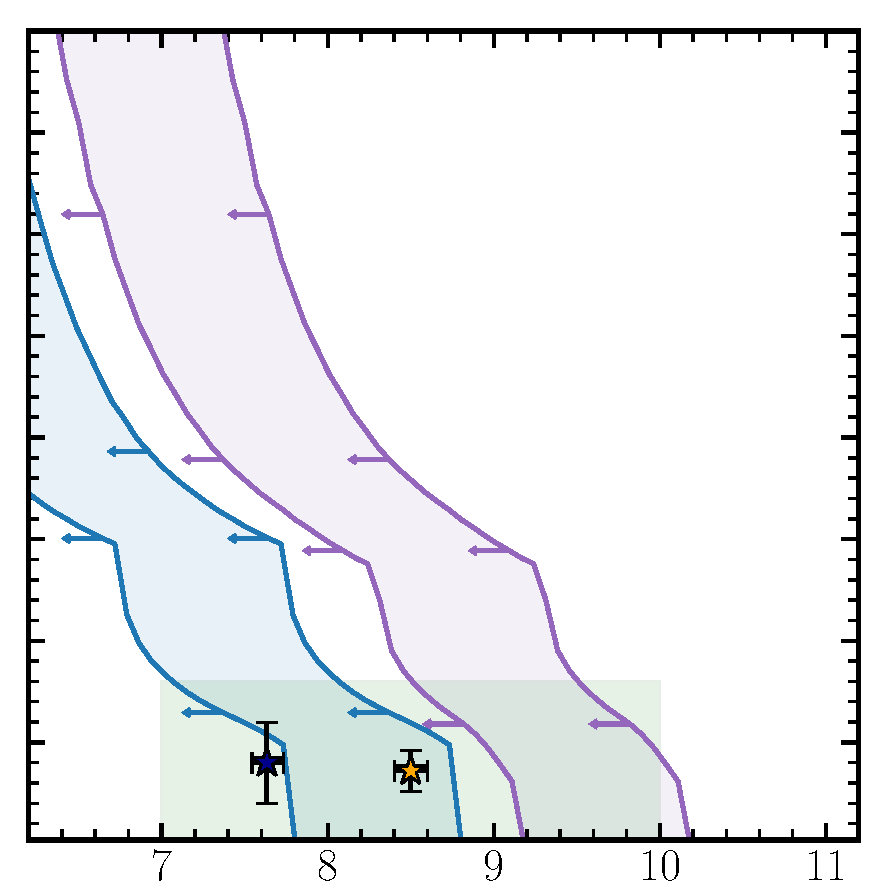
\includegraphics[width=\linewidth,height=6.6cm,keepaspectratio]{assets/comparison/fig5_eff_stellar_original.pdf}
\end{minipage}
\end{column}
\begin{column}{.485\textwidth}
\centering\textbf{复现结果}\\[1mm]
\begin{minipage}[c][6.65cm][c]{\linewidth}\centering
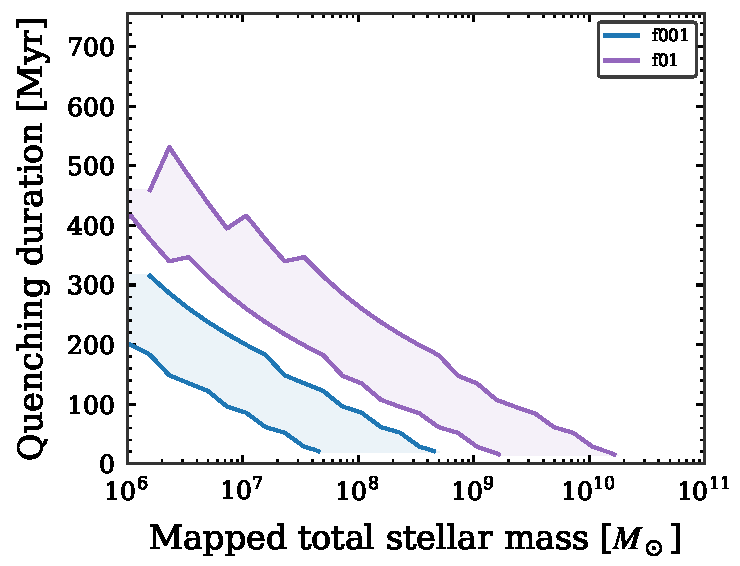
\includegraphics[width=\linewidth,height=6.6cm,keepaspectratio]{assets/comparison/fig5_eff_stellar_computed.pdf}
\end{minipage}
\end{column}
\end{columns}
\vspace{1mm}
{\fontsize{10}{13}\selectfont $M_{\star,\rm tot}=\tilde f_\star f_bM_h$，$\tilde f_\star=0.01$--0.1；这不是本轮形成质量。右图为 SN-only。\par}
\src{原图 Fig. 5 对应面板裁切；左右纵轴范围不同。右侧叉号为未启动、红短线为失败、三角为未返回下限。}
\end{frame}
\begin{frame}[t]{图 5：IMF 与暗晕质量}
\par
\begin{columns}[T,onlytextwidth]
\begin{column}{.485\textwidth}
\centering\textbf{论文原图}\\[1mm]
\begin{minipage}[c][6.65cm][c]{\linewidth}\centering
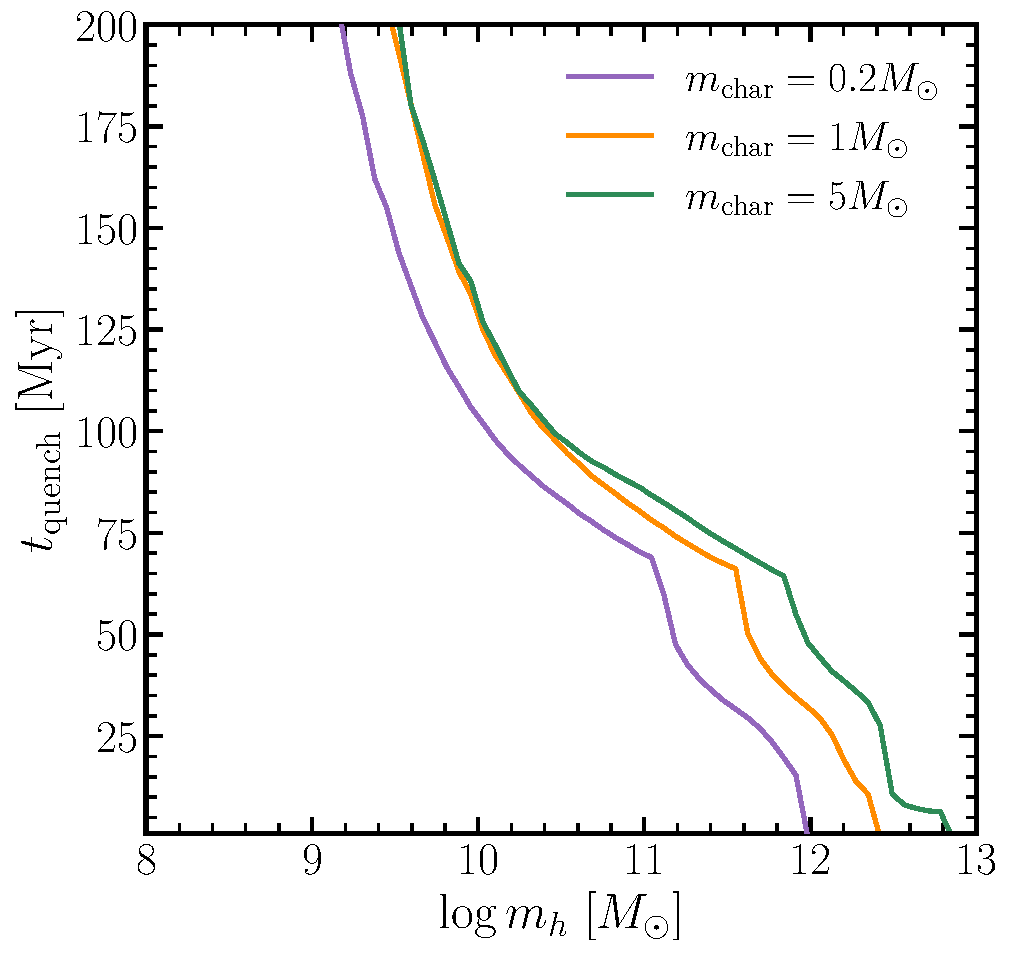
\includegraphics[width=\linewidth,height=6.6cm,keepaspectratio]{assets/comparison/fig5_imf_halo_original.pdf}
\end{minipage}
\end{column}
\begin{column}{.485\textwidth}
\centering\textbf{复现结果}\\[1mm]
\begin{minipage}[c][6.65cm][c]{\linewidth}\centering
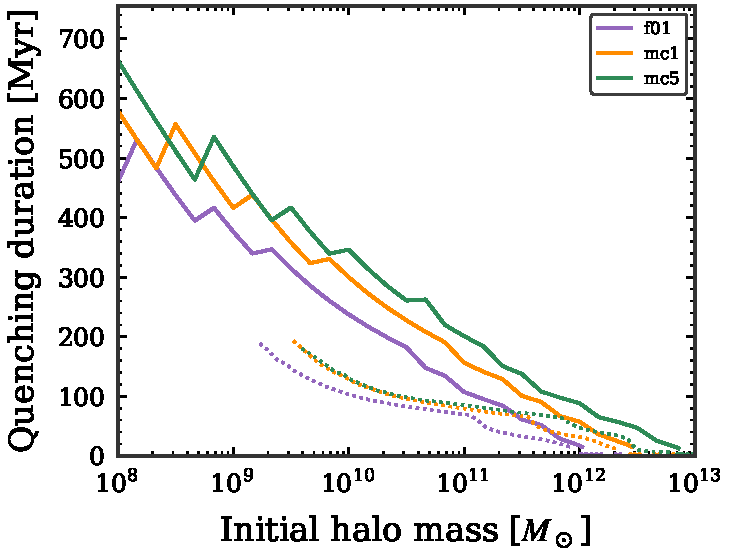
\includegraphics[width=\linewidth,height=6.6cm,keepaspectratio]{assets/comparison/fig5_imf_halo_computed.pdf}
\end{minipage}
\end{column}
\end{columns}
\vspace{1mm}
{\fontsize{10}{13}\selectfont $f_\star=0.01$；右图 f01/mc1/mc5 对应 $m_{\rm char}=0.2/1/5\,M_\odot$，均为 SN-only。\par}
\src{原图 Fig. 5 对应面板裁切；左右纵轴范围不同。右侧叉号为未启动、红短线为失败、三角为未返回下限。}
\end{frame}
\begin{frame}[t]{图 5：IMF 与观测恒星质量映射}
\par
\begin{columns}[T,onlytextwidth]
\begin{column}{.485\textwidth}
\centering\textbf{论文原图}\\[1mm]
\begin{minipage}[c][6.65cm][c]{\linewidth}\centering
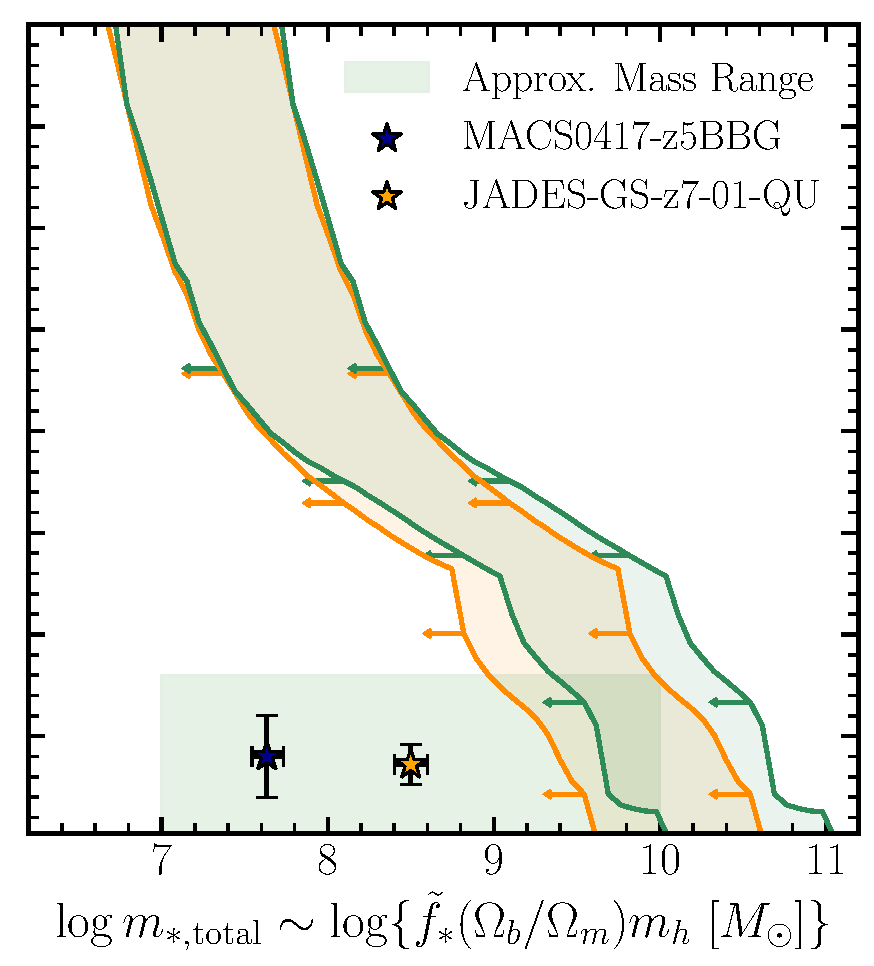
\includegraphics[width=\linewidth,height=6.6cm,keepaspectratio]{assets/comparison/fig5_imf_stellar_original.pdf}
\end{minipage}
\end{column}
\begin{column}{.485\textwidth}
\centering\textbf{复现结果}\\[1mm]
\begin{minipage}[c][6.65cm][c]{\linewidth}\centering
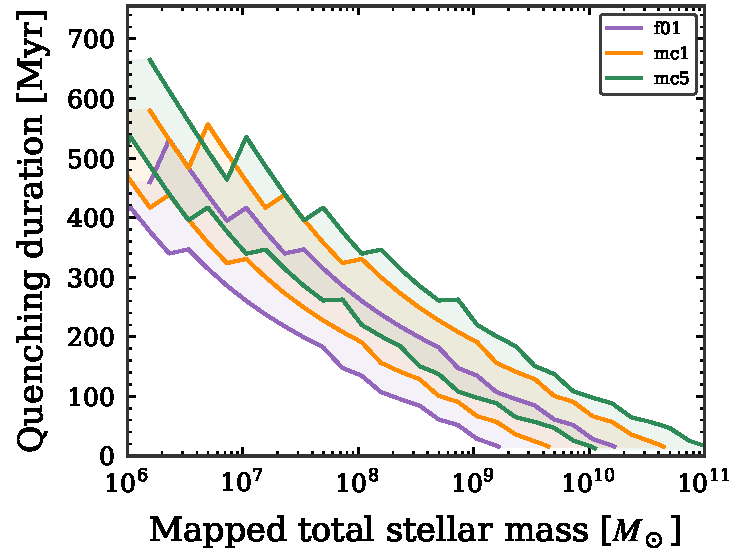
\includegraphics[width=\linewidth,height=6.6cm,keepaspectratio]{assets/comparison/fig5_imf_stellar_computed.pdf}
\end{minipage}
\end{column}
\end{columns}
\vspace{1mm}
{\fontsize{10}{13}\selectfont 右图为 SN-only 及独立净效率映射；原图中的观测点保留于左侧，右侧未添加无来源观测数值。\par}
\src{原图 Fig. 5 对应面板裁切；左右纵轴范围不同。右侧叉号为未启动、红短线为失败、三角为未返回下限。}
\end{frame}
\begin{frame}[t]{图 8：吸积覆盖率与初始气体，$f_\star=0.001$}
\par
\begin{columns}[T,onlytextwidth]
\begin{column}{.485\textwidth}
\centering\textbf{论文原图}\\[1mm]
\begin{minipage}[c][6.65cm][c]{\linewidth}\centering
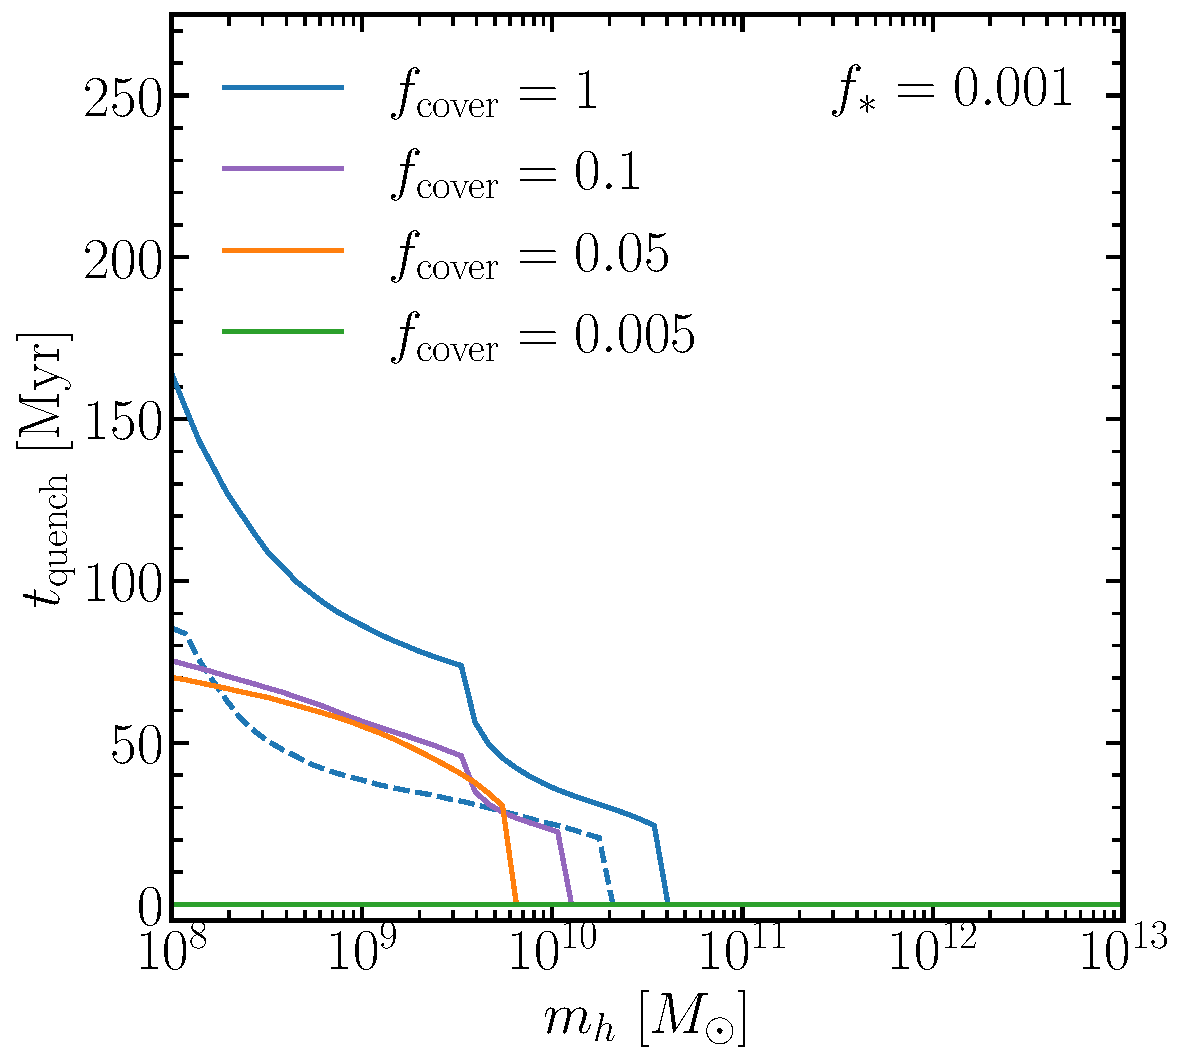
\includegraphics[width=\linewidth,height=6.6cm,keepaspectratio]{assets/comparison/fig8_f001_original.pdf}
\end{minipage}
\end{column}
\begin{column}{.485\textwidth}
\centering\textbf{复现结果}\\[1mm]
\begin{minipage}[c][6.65cm][c]{\linewidth}\centering
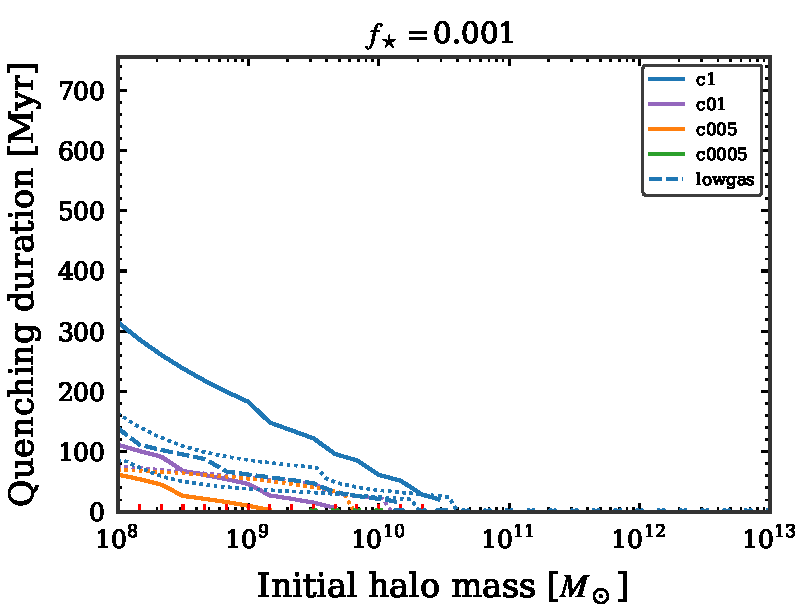
\includegraphics[width=\linewidth,height=6.6cm,keepaspectratio]{assets/comparison/fig8_f001_computed.pdf}
\end{minipage}
\end{column}
\end{columns}
\vspace{1mm}
{\fontsize{10}{13}\selectfont $\dot M_{\rm acc}=f_b\dot M_h$ 不随覆盖率缩减；lowgas 仅减少初始储库。右图为 SN-only，点线为原图。\par}
\src{原图 Fig. 8 对应面板裁切；左右纵轴范围不同。c1/c01/c005/c0005 对应 $f_{\rm cover}=1/0.1/0.05/0.005$。}
\end{frame}
\begin{frame}[t]{图 8：吸积覆盖率与初始气体，$f_\star=0.01$}
\par
\begin{columns}[T,onlytextwidth]
\begin{column}{.485\textwidth}
\centering\textbf{论文原图}\\[1mm]
\begin{minipage}[c][6.65cm][c]{\linewidth}\centering
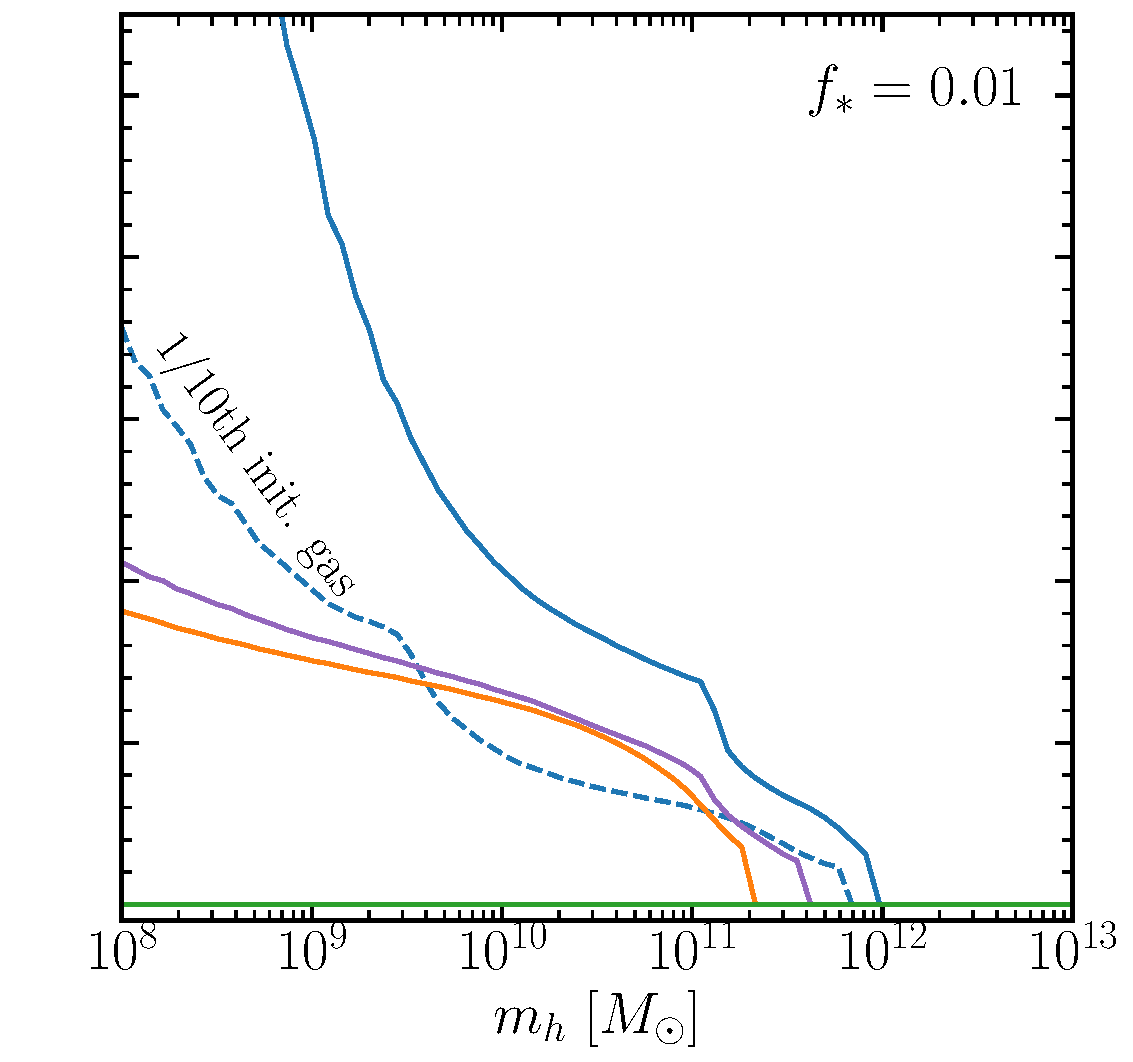
\includegraphics[width=\linewidth,height=6.6cm,keepaspectratio]{assets/comparison/fig8_f01_original.pdf}
\end{minipage}
\end{column}
\begin{column}{.485\textwidth}
\centering\textbf{复现结果}\\[1mm]
\begin{minipage}[c][6.65cm][c]{\linewidth}\centering
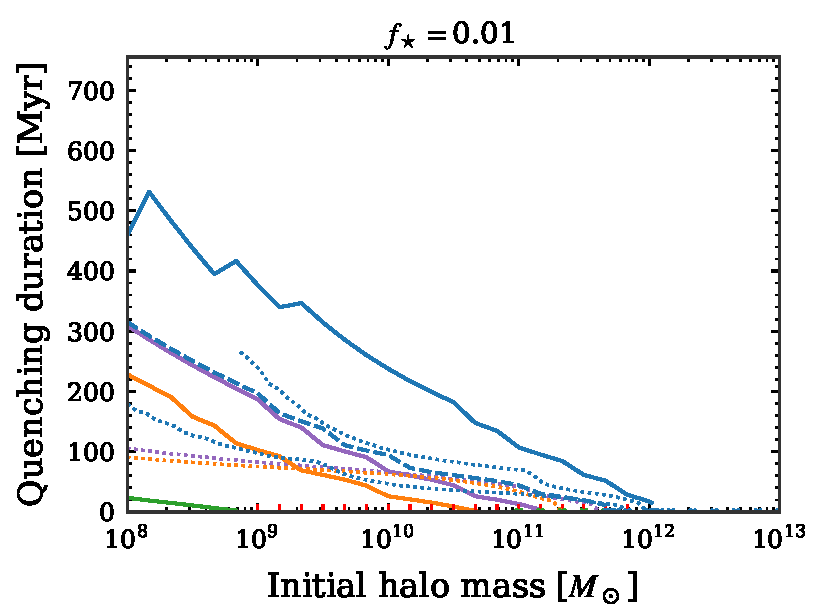
\includegraphics[width=\linewidth,height=6.6cm,keepaspectratio]{assets/comparison/fig8_f01_computed.pdf}
\end{minipage}
\end{column}
\end{columns}
\vspace{1mm}
{\fontsize{10}{13}\selectfont $\dot M_{\rm acc}=f_b\dot M_h$ 不随覆盖率缩减；lowgas 仅减少初始储库。右图为 SN-only，点线为原图。\par}
\src{原图 Fig. 8 对应面板裁切；左右纵轴范围不同。c1/c01/c005/c0005 对应 $f_{\rm cover}=1/0.1/0.05/0.005$。}
\end{frame}
\begin{frame}[t]{数值精度不能解释论文曲线的巨大差异}
\par
\begin{tabular}{lll}
\toprule 检查 & 实测 & 解释\\\midrule
pytest & 24 项通过 & IMF、历史反馈、能量/动量、事件\\
代表轨道收敛 & 三指标变化 $<0.02\%$ & $10^8$ 全项近似、$10^9$ SN-only\\
临界质量收敛 & $[2.8741,2.8822]\times10^{10}M_\odot$ & SN-only，三个历史格距\\
全反馈 full & 41.9 s & 26 完成、156 未启动、285 失败\\
SN-only full & 71.2 s & 276 完成、177 未启动、41 失败、5 下限\\\bottomrule
\end{tabular}

缺失的作者约定：恒星半径、壳层温度/密度闭合、形成区释放条件、回落加载及图 4 数值 SFH。

下一步需要这些原始实现证据；不能把未决细节改成任意常数后宣布复现成功。
\src{全部机器可读曲线、失败原因、配置、计时、收敛表与日志均保存在独立项目中。}
\end{frame}
\end{document}
